\documentclass[titlepage]{article}
\setlength{\parskip}{1.5pt}
\setlength{\parindent}{0cm}
\usepackage{amsmath, amsfonts, graphicx, subcaption}
%Path relative to the main .tex file 
\graphicspath{ {./Imagenes/} }


\title{Ejercicio 2: EDP Forward de Black - Scholes}
\author{Los del Grupo 2}
\date{\today}

\begin{document}
\maketitle

En la EDP de Black-Scholes, teniendo en cuenta que el subyacente evoluciona según el proceso: \\

$dS(t) = rS(t)dt + \sigma(S,t)dW(t)$ \\

$\sigma(S,t) = \sigma S^{\beta}(t)$  \\

Implementar: \\

\begin{itemize}
	\item Si $\beta = 0.8$, un esquema totalmente implícito con condiciones de Neumann: \\
		\begin{center}
			en los bordes: $S_{min} = 0, S_{max} = 4 \cdot S_{0}$ y $\dfrac{\partial^{2}u}{\partial{x}^{2}} = 0$
		\end{center}
		
	\item Además, para el mismo valor de $\beta$, comprobar el resultado para el último vencimiento implementado en un esquema de diferencias finitas implícito en la ecuación backward.
	
	\item Smile generado: para los valores de $\beta$ 0.7, 0.8, 0.9, obtener las volatilidades implícitas para los distintos strikes que genera el modelo en los vencimientos 1 mes, 3 meses y 6 meses. Graficar los tres vencimientos por separado.
	
	\item Ahora supongamos que estamos valorando un derivado que tiene un pago de un cupón determinista y conocido (por ejemplo 1$\%$) antes del vencimiento, redactar por escrito como se implementaría este pago discreto en un esquema de diferencias finitas.	
\end{itemize}

Datos: \\

\begin{tabular}{| l | c |}
	\hline
		T & 6 meses \\
		r & 1 $\%$ \\
		$S_{0}$ & 9 \\
		K & 8 \\
		$\sigma$ & 50$\%$\\
	\hline	
\end{tabular}

\newpage
\subsubsection*{EDP Forward}

Para definir el esquema forward, nos apoyaremos en el Teorema Fundamental de Valoración, el cual establece lo siguiente:

\begin{center}
	$c(T,K) = \dfrac{C(T,K)}{B(t,T)} = E_{\mathbb{Q}}[(S_{T} - K)^{+} \mid \mathcal{F}_{t}]$
\end{center}

Tomaremos el proceso $X_{T} := (S_{T} - K)^{+}$, sobre el cual aplicaremos Ito para obtener la siguiente evolución:

\begin{center}
	$dX_{T} = \dfrac{\partial X_{T}}{\partial S_{T}} dS_{T} + \dfrac{1}{2} \dfrac{\partial^{2} X_{T}}{\partial S_{T}^{2}}(dS_{T})^{2}$
\end{center}

Esto se puede definir del siguiente modo:

\begin{center}
	$dX_{T} = 1_{(S_{T} > K)} r S_{T} dT + \dfrac{1}{2} \partial (S_{T} - K) \sigma^{2}S_{T}^{2\beta}dT + 1_{(S_{T} > K)} \sigma S_{T}^{\beta} dW_{T}^{\mathbb{Q}}$
\end{center}

A partir de aquí, seguiremos un proceso análogo al definido en las notas de clase para poder obtener una ecuación forward para la EDP de Black - Scholes, es decir, procederemos a integrar la formula anterior entre \textit{t} y \textit{T}, para posteriormente tomar valores esperados condicionados a la filtración $\mathcal{F}_{t}$, con esto obtendremos la siguiente formula para nuestro derivado:

\begin{center}
	$c(T,K) - c(t, K) = \displaystyle \int_{t}^{T} r_{h} (c(h, K) - K \dfrac{\partial c(T,K)}{\partial K}) dh + \dfrac{1}{2} \int_{t}^{T} \sigma_{h}(K)^{2} \dfrac{\partial^{2}c(h, K)}{\partial K^{2}} dh$
\end{center}

Finalmente, derivando con respecto a T, obtendremos la EDP forward de Black - Scholes:

\begin{center}
	$\dfrac{\partial c(T, K)}{\partial T} - r_{T} c(T, K) + r_{T}K \dfrac{\partial c(T, K)}{\partial K} - \dfrac{1}{2} \sigma_{T}^{2}K^{2 \beta} \dfrac{\partial^{2}c(T, K)}{\partial^{2}K} = 0$
\end{center}

Podemos apreciar que el signo de la derivada de segundo orden con respecto al strike $(K)$ es negativa. Esto permite entender que estamos ante una EDP forward, y que por lo tanto, requiere de la fijación de una condición inicial, en este caso se ha fijado:

\begin{center}
	$c(t, K) = (S_{t} - K)^{+}$
\end{center}

Una vez que tenemos las condición inicial, recordando las condiciones de contorno del estilo Neummann:

\begin{center}
	$\dfrac{\partial^{2}u}{\partial{x}^{2}} = 0$
\end{center}

Vamos a definir un esquema implícito de diferencias finitas para poder obtener los valores de la EDP. Lo siguiente es una representación esquemática del proceso:

\begin{center}
	\begin{tabular}{ l c c r }
	\hline
		$x_{j+1}$ & $\circ$ & & $\circ$ \\
		 & & & $\downarrow$ \\
		$x_{j}$ & $\circ$ & $\longrightarrow$ & $\circ$ \\
		 & & & $\uparrow$ \\
		$x_{j-1}$ & $\circ$ &  & $\circ$ \\		
		 & $t_{i-1}$ &  &$t_{i}$ \\	
	\hline	
	\end{tabular}
\end{center}

Para facilitar el desarrollo y mejorar el entendimiento del proceso vamos a apoyarnos en las siguientes definiciones (el objetivo es aproximarnos a la notación definida en las notas facilitadas en clase).

\begin{itemize}
	\item[] $a(x, t) = -\dfrac{1}{2} \sigma^{2} x^{2\beta}$ 
	\item[] $b(x, t) = rx$
	\item[] $c(x, t) = -r$	
\end{itemize}

Una vez definidos estos elementos, la EDP a calcular tiene la siguiente forma:

\begin{center}
	$\dfrac{\partial u}{\partial t} + a(x, t) \dfrac{\partial^{2}u}{\partial{x}^{2}} + b(x, t) \dfrac{\partial u}{\partial x} + c(x, t) u = 0$
\end{center}

Puesto que la ecuación es forward, iremos resolviendo la ecuación hacia delante en la variable temporal, por lo cual, expresaremos las derivadas parciales del siguiente modo para discretizar la ecuación:

\begin{itemize}
	\item[] $\dfrac{\partial u}{\partial t} \approx \dfrac{u_{i+1}(j) - u_{i}(j)}{\Delta t}$
	\item[] $\dfrac{\partial^{2}u}{\partial{x}^{2}} \approx \dfrac{u_{i+1}(j+1) - 2u_{i}(j) + u_{i+1}(j-1)}{(\Delta x)^2}$
	\item[] $\dfrac{\partial u}{\partial x} \approx \dfrac{u_{i+1}(j+1) - u_{i+1}(j-1)}{2 \Delta x}$
\end{itemize}

Por lo cual, obtenemos la siguiente versión discreta de la EDP forward de Black - Scholes:

\begin{center}
	$\dfrac{u_{i+1}(j) - u_{i}(j)}{\Delta t} + a_{i+1}(j) \dfrac{u_{i+1}(j+1) - 2u_{i}(j) + u_{i+1}(j-1)}{(\Delta x)^2} + b_{i+1}(j) \dfrac{u_{i+1}(j+1) - u_{i+1}(j-1)}{2 \Delta x} + c_{i+1}(j) u_{i+1}(j) = 0$
\end{center}

Definiremos los siguientes valores:

\begin{itemize}
	\item[] $\alpha = \dfrac{\Delta t}{(\Delta x)^{2}}$
	\item[] $\rho = \dfrac{\Delta t}{\Delta x}$
\end{itemize}

Operando obtenemos:
\begin{center}
	\begin{multline*}
		u_{i+1}(j) - u_{i}(j) + \alpha a_{i+1}(j) [u_{i+1}(j+1) - 2u_{i+1}(j) + u_{i+1}(j-1)] \\
		 + \dfrac{\rho}{2} b_{i+1}(j) [u_{i+1}(j+1) - u_{i+1}(j-1)] + \Delta t c_{i+1}(j) u_{i+1}(j) = 0
	\end{multline*}
	\begin{align*}
		u_{i}(j) &=  u_{i+1}(j+1)[\alpha a_{i+1}(j) + \dfrac{\rho}{2} b_{i+1}(j)] \\ 
		& + u_{i+1}(j)[1 - 2  \alpha a_{i+1}(j) + \Delta t c_{i+1}(j)] \\
		& + u_{i+1}(j-1) [\alpha a_{i+1}(j) - \dfrac{\rho}{2} b_{i+1}(j)]
	\end{align*}

\end{center}

Esta ecuación nos permitirá definir un sistema de ecuaciones con el cual ir resolviendo de forma iterativa el calculo para cada uno de los nodos, avanzando en el espacio temporal, el problema es que tal y como está definido, se puede observar que existen dos puntos que dependen de valores que se encuentran fuera del mallado, como desconocemos estos puntos, vamos a utilizar las condiciones de contorno de Neummann para poder eliminar esta dependencia y así poder calcular los valores. Para ello, cabe recordar que vamos a fijar que nuestra función en ambos extremos cumpla la siguiente condición:

\begin{center}
	$\dfrac{\partial^{2}u}{\partial{x}^{2}} = 0$
\end{center}

Esto hace que:

\begin{center}
	$\dfrac{u_{i+1}(j+1) - 2u_{i}(j) + u_{i+1}(j-1)}{(\Delta x)^2} = 0$
\end{center}

Resolviendo dicha ecuación obtenemos:
\begin{align*}
	u_{i+1}(m) &= 2u_{i+1}(m-1) - u_{i+1}(m-2)\\
	u_{i+1}(0) &= 2u_{i+1}(1) - u_{i+1}(2)
\end{align*}
	
Utilizaremos ambos elementos para poder definir correctamente la matriz que nos servirá para calcular de forma iterativa el valor de la EDP forward de Black - Scholes. Para ello vamos a redefinir el punto \textit{j = 1} y el punto \textit{j = m - 1}

\begin{itemize}
	\item \textbf{j = 1}
		\begin{align*}
			u_{i}(1) &= u_{i+1}(2)[\alpha a_{i+1}(1) + \dfrac{\rho}{2} b_{i+1}(1)] \\
			& + u_{i+1}(1)[1 - 2 \alpha	a_{i+1}(1) + \Delta t c_{i+1}(1)] \\
			& + u_{i+1}(0)[\alpha a_{i+1}(1) - \dfrac{\rho}{2} b_{i+1}(1)]
		\end{align*}
		
	Sabiendo que: $u_{i+1}(0) = 2u_{i+1}(1) - u_{i+1}(2)$ \\
	
	Obtenemos:
		\begin{center}
			$u_{i}(1) = u_{i+1}(2)[\rho b_{i+1}(1)] + u_{i+1}(1)[1 + \Delta t c_{i+1}(1) - \rho b_{i+1}(1)]$
		\end{center}
		
	\item \textbf{j = m - 1}
		\begin{align*}
			u_{i}(m - 1) &= u_{i+1}(m)[\alpha a_{i+1}(m - 1) + \dfrac{\rho}{2} b_{i+1}(m - 1)] \\
			& + u_{i+1}(m - 1)[1 - 2 \alpha	a_{i+1}(m - 1) + \Delta t c_{i+1}(m - 1)] \\
			& + u_{i+1}(m - 2)[\alpha a_{i+1}(m - 1) - \dfrac{\rho}{2} b_{i+1}(m - 1)]
		\end{align*}
		
	Sabiendo que: $u_{i+1}(m) = 2u_{i+1}(m - 1) - u_{i+1}(m - 2)$ \\
	
	Obtenemos:
		\begin{align*}
			u_{i}(m - 1) &= \\
			& u_{i+1}(m - 1)[1 + \Delta t c_{i+1}(m - 1) - \rho b_{i+1}(m - 1)] + u_{i+1}(m - 2)[-\rho b_{i+1}(m - 1)]
		\end{align*}

\end{itemize}

Con esto podemos definir la siguiente matriz:

\begin{center}
$$ M^{i+1} = 
	\begin{pmatrix}
		diag_{i+1}(1) & up_{i+1}(1) & \cdots & \cdots \\
		low_{i+1}(2) & diag_{i+1}(2) & up_{i+1}(2) & \cdots \\
		\vdots  & \vdots  & \ddots & \vdots  \\
		\vdots  & \vdots  & low_{i+1}(m - 1) & diag_{i+1}(m - 1) \\ 
	\end{pmatrix}
$$
\end{center}

Que nos permitirá resolver para los tiempos \textit{i = 0, 1, ..., n - 1, n}, de forma iterativa, el siguiente sistema lineal:

\begin{align*}
	M^{i+1}u_{i+1} &= u_{i} \\
	u_{i+1} &= (M^{i+1})^{-1} u_{i}
\end{align*}

Hay que recordar, que el valor en los bordes será obtenido gracias a la condición de contorno de Neummann, con las que se han definido las siguientes ecuaciones: 

\begin{align*}
	u_{i+1}(m) &= 2u_{i+1}(m-1) - u_{i+1}(m-2)\\
	u_{i+1}(0) &= 2u_{i+1}(1) - u_{i+1}(2)
\end{align*}

Dentro del archivo Excel "Ejercicio 2" (en la pestaña Forward) y el notebook "Notebook$\_$Ejercicio$\_$2.ipynb" adjuntos, se han implementado la solución. Se pueden modificar los parámetros para poder ver las sensibilidades, por ejemplo a las variaciones de $\beta$. Las pequeñas diferencias que hemos encontrado entre ambos archivos consideramos que se deben a diferencias numéricas, ya que los resultados empiezan a discrepar a partir del tercer decimal.

\vspace{5pt}
En la imagen \ref{fig: EDP Forward} podemos observar ambas gráficas de superficie:

\begin{figure}
	\begin{subfigure}{7cm}
    	\centering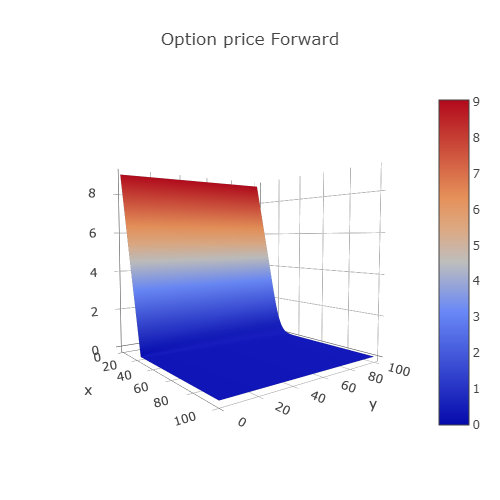
\includegraphics[width=6cm]{PyEDPForward}
  	\end{subfigure}
  	\begin{subfigure}{7cm}
    	\centering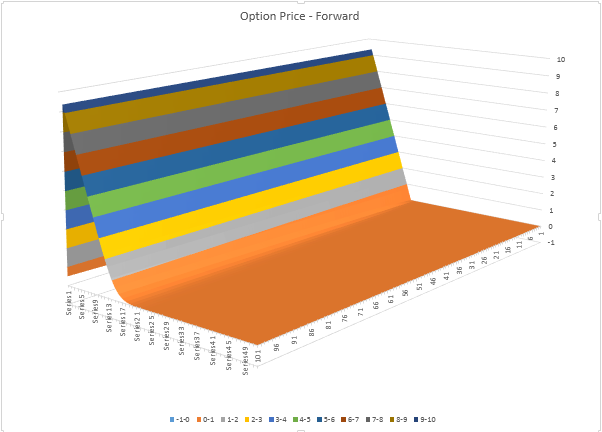
\includegraphics[width=6cm]{ExEDPForward}
  	\end{subfigure}
  	\caption{Precio de Opción con EDP Forward con Python (izq) y Excel (der)}
  	\label{fig: EDP Forward}
\end{figure}

\newpage
\subsubsection*{EDP Backward}

La segunda parte del ejercicio nos pide, fijando el valor de $\beta$, comprobar el resultado implementando un esquema de diferencias finitas para la ecuación backward. Esta ecuación tiene la siguiente forma:

\begin{center}
	$\dfrac{\partial u}{\partial t} + a(x, t) \dfrac{\partial^{2}u}{\partial{x}^{2}} + b(x, t) \dfrac{\partial u}{\partial x} + c(x, t) u = 0$
\end{center}

Con los siguientes parámetros:

\begin{itemize}
	\item[] $a(x, t) = \dfrac{1}{2} \sigma^{2} S_{t}^{2\beta}$ 
	\item[] $b(x, t) = rS_{t}$
	\item[] $c(x, t) = -r$	
\end{itemize}

En este caso, podemos observar que es una EDP backwards, por que el signo de la segunda derivada con respecto al subyacente ($S_{t}$) es positivo, por lo tanto, necesitaremos una condición final, que junto a las condiciones de contorno, otra vez impondremos la condición Neummann sobre la segunda derivada con respecto al subyacente, nos permitirá crear un esquema de diferencias finitas implícito para poder resolverla y utilizar los resultados obtenidos para comparar y comprobar ambas soluciones.

\vspace{7pt}
Condición final:
\begin{center}
	$c(T, K) = (S_{T} - K)^{+}$
\end{center}

Condición de contorno Neummann:

\begin{center}
	$\dfrac{\partial^{2}u}{\partial{x}^{2}} = 0$
\end{center}

No vamos a extendernos en el desarrollo de las diferencias finitas para esta ecuación, ya que ha sido visto en clase, simplemente procederemos a definir aquí la version discreta de la EDP backwards de Black - Scholes:

\begin{center}
	$\dfrac{u_{i}(j) - u_{i-1}(j)}{\Delta t} + a_{i-1}(j) \dfrac{u_{i-1}(j+1) - 2u_{i-1}(j) + u_{i-1}(j-1)}{(\Delta x)^2} + b_{i-1}(j) \dfrac{u_{i-1}(j+1) - u_{i-1}(j-1)}{2 \Delta x} + c_{i-1}(j) u_{i-1}(j) = 0$
\end{center}

Operando y reorganizando obtenemos:
\begin{align*}
	u_{i}(j) &=  u_{i-1}(j+1)[-\alpha a_{i-1}(j) + \dfrac{\rho}{2} b_{i-1}(j)] \\ 
	& + u_{i-1}(j)[1 + 2  \alpha a_{i+1}(j) - \Delta t c_{i+1}(j)] \\
	& + u_{i-1}(j-1) [-\alpha a_{i+1}(j) - \dfrac{\rho}{2} b_{i+1}(j)]
\end{align*}

En este caso, llegamos también a un sistema lineal de ecuaciones de la siguiente forma:

\begin{align*}
	M^{i-1}u_{i-1} &= u_{i} \\
	u_{i-1} &= (M^{i-1})^{-1} u_{i}
\end{align*}

Que se resolverá de forma iterativa, para los tiempos \textit{i = n, n - 1, ..., 1, 0}. Por lo tanto, en este caso, partiendo de la condición final, en tiempo \textit{n}, vamos resolviendo el sistema "hacia atrás".

\vspace{5pt}
Dentro del archivo Excel "Ejercicio 2" (en la pestaña Forward) y el notebook "Notebook$\_$Ejercicio$\_$2.ipynb" adjuntos, se han implementado la solución. Se pueden modificar los parámetros para poder ver las sensibilidades, por ejemplo a las variaciones de $\beta$. Las pequeñas diferencias que hemos encontrado entre ambos archivos consideramos que se deben a diferencias numéricas, ya que los resultados empiezan a discrepar a partir del tercer decimal.

\vspace{5pt}
En la imagen \ref{fig: EDP Backward} podemos observar ambas gráficas de superficie.

\begin{figure}[h]
	\begin{subfigure}{7cm}
    	\centering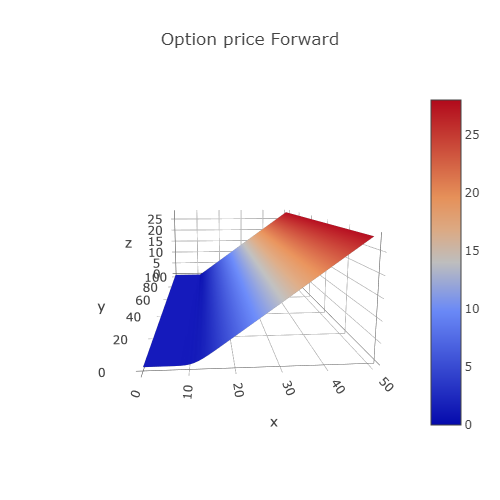
\includegraphics[width=6cm]{PyEDPBackward}
  	\end{subfigure}
  	\begin{subfigure}{7cm}
    	\centering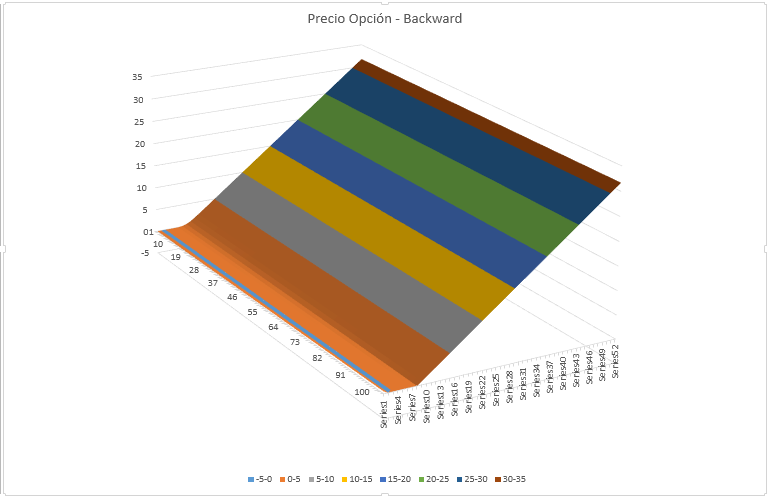
\includegraphics[width=6cm]{ExEDPBackward}
  	\end{subfigure}
  	\caption{Precio de Opción con EDP Backward con Python (izq) y Excel (der)}
  	\label{fig: EDP Backward}
\end{figure}

\vspace{5pt}
Finalmente, para poder realizar la comprobación se ha montado tanto en el Excel "Ejercicio 2" (en la pestaña Backwards) y el notebook "Notebook$\_$Ejercicio$\_$2.ipynb" adjuntos, un esquema implícito de la EDP backwards, en ambos casos se puede comprobar que fijado el mismo $\beta$, y para un spot del subyacente de 9, seleccionaremos 3 valores de strike distintos, podemos comprobar como es posible recuperar el precio aplicando la EDP forward y backwards \footnote{Se han incluido los resultados del "Notebook$\_$Ejercicio$\_$2.ipynb"}.

\begin{center}
	\begin{tabular}{c c c c c}
	\hline
	Subyacente & $\beta$ & Strike & Valor EDP Forward & Valor EDP Backward \\
	\hline 
	9 & 0.7 & 2.159 & 6.885 & 6.850 \\
	9 & 0.7 & 4.319 & 4.725 & 4.701 \\
	9 & 0.7 & 5.760 & 3.290 & 3.273 \\	
	\hline
	\end{tabular}
\end{center} 

\newpage
\subsubsection*{Smile}

La tercera parte del ejercicio, nos solicita obtener las volatilidades implícitas para valores de $\beta$ de 0.7, 0.8 y 0.9 de los distintos strikes (por tanto de la EDP forward) para vencimientos de 1 mes, 3 meses y 6 meses. Para obtener dicha volatilidad implícita, se invierte la función de Black - Scholes para opciones call a los vencimientos definidos, esto nos permitirá recuperar la volatilidad implícita, es decir, la volatilidad que al ser incluida como input en el modelo de Black - Scholes (que asume volatilidad constante), replica el valor de la call obtenido. Al fijar los vencimientos obtendremos la curva del smile de volatilidad. En este caso hemos obtenido las volatilidades implícitas mediante algoritmos que minimizan la diferencia entre el valor obtenido con el modelo de Black - Scholes, y el valor obtenido mediante la resolución de la EDP. 

\vspace{5pt}
Se puede observar que el punto de inflexión de la gráfica se suele encontrar en torno al precio spot del subyacente que hemos fijado.

\begin{figure}[h]
	\centering
	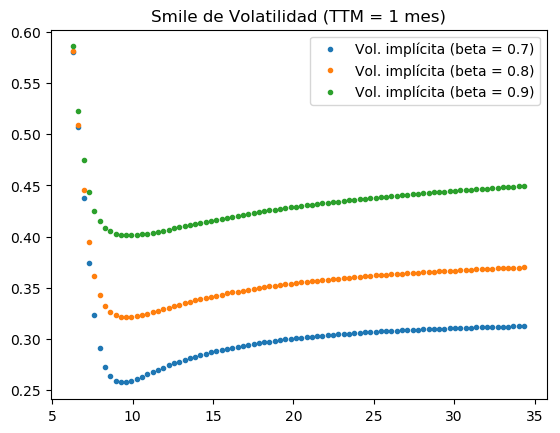
\includegraphics[scale=0.65]{TTM1}
	\caption{TTM = 1 mes}
\end{figure}

\begin{figure}[!]
	\centering
	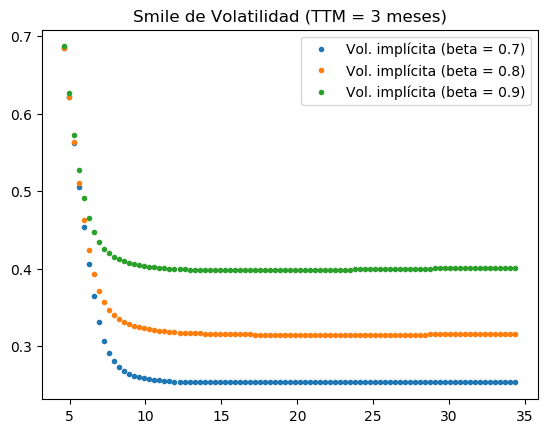
\includegraphics[scale=0.65]{TTM3}
	\caption{TTM = 3 mes}
\end{figure}

\begin{figure}[!]
	\centering
	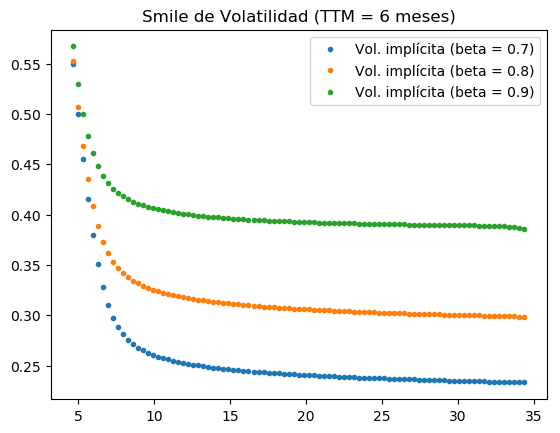
\includegraphics[scale=0.65]{TTM6}
	\caption{TTM = 6 mes}
\end{figure}

\newpage
\subsubsection*{Derivado que tiene un pago de un cupón determinista y conocido antes del vencimiento}

Dado que se trata de un pago conocido, la EDP a resolver para obtener el precio del derivado (V) se reduce a la siguiente expresión:

\begin{center}
	$\dfrac{\partial V_{t}}{\partial t} = rV$
\end{center}

Donde \textit{r} es el tipo de interés (que suponemos constante).

\vspace{5pt}
Sea \textit{T} el vencimiento del derivado, $t_{p}$ el tiempo de pago del cupón y $t_{0}$ el tiempo inicial. Supondremos que $t_{0}=0$. Notemos que la relación entre estos tiempos es: $t_{0} \leq t_{p} \leq T$.  

\vspace{5pt}
Sabemos que la solución analítica, obtenida resolviendo la ecuación, es la siguiente (integrando entre t y T):

\begin{align*}
	\dfrac{\partial V_{t}}{\partial t} &= rV \\
	\dfrac{\partial V_{t}}{V} &= r\partial t \\
	ln(V_{T}) - ln(V_{t}) &= \displaystyle \int_{t}^{T} r\partial t\\
	ln(V_{T}) &= ln(V_{t}) + r(T - t) \\
	V_{T} &= V_{t}\exp^{r(T-t)} \\
	V_{t} &= V_{T} \exp^{-r(T-t)} \\
\end{align*}

Sea \textit{C} el pago del cupón (1$\%$ por el nominal si seguimos el ejemplo del enunciado). Tenemos la condición de que $V_{t_{p}} = C$. Por lo que:

\begin{center}
	$C = V_{t_{p}} = V_{T} \exp^{-r(T-t_{p})} \longrightarrow V_{T} = C\exp^{r(T-t_{p})} \longrightarrow V_{t} = V_{T} \exp^{-r(t_{p}-t)} $
\end{center}
	
Para todo \textit{t} entre \textit{0} y \textit{T}. Si queremos valorar el derivado en  \textit{t} = 0, se tiene:

\begin{center}
	$V_{0} = C\exp^{-rt_{p}}$
\end{center}

Veamos cómo implementar este pago por un esquema de diferencias finitas. Dado que tenemos una condición “intermedia” una posible solución es implementar un esquema backward para valores de \textit{t} entre 0 y $t_{p}$, y un esquema forward para valores de \textit{t} entre $t_{p}$ y  \textit{T}. Veamos cómo quedaría los diferentes esquemas tanto para la parte backward como para la parte forward. 

\vspace{5pt}
Como \textit{V} sólo tiene dependencia temporal se realiza un mallado espaciador únicamente en una dimensión. En este caso consideraremos un mallado para el lado de la backward y otro para el de la forward.

\begin{itemize}
	\item[\textbf{a)}] \textbf{Backward:} Tomamos un mallado de $N_{1}$ puntos entre $t_{0} = 0$ y $t_{p}$. Es decir, compuesto por $\left\lbrace t_{i} \right\rbrace_{i = 0}^{N_{1}}$ donde $t_{i} = t_{0} + i \Delta t \forall i$. Sea $\Delta t = \dfrac{t_{p}}{N_{1}}$ 
	
	\item[\textbf{b)}] \textbf{Forward:} Tomamos un mallado de $N_{2}$ puntos entre $t_{p}$ y \textit{T}. Es decir, compuesto por $\left\lbrace t_{j} \right\rbrace_{j = 0}^{N_{2}}$ donde $t_{j} = t_{p} + j \overline{\Delta t} \forall j$. Sea $\overline{\Delta t} = \dfrac{t_{p}}{N_{1}}$ 
\end{itemize}

A continuación denotaremos por \textit{V} al valor del derivado para la parte Backward y $\overline{V}$ para la parte Forward.

\begin{itemize}
	\item \textbf{Esquema explícito}

	\vspace{5pt}
	Partimos de:
		\begin{center}
			$\dfrac{V(i) - V(i-1}{\Delta t} = r V(i)$
		\end{center}
	
	Despejando, se obtienen los siguientes esquemas para Backward y Forward, respectivamente:
		\begin{align*}
			V(i - 1) &= (1 - r \Delta t)V(i) \\
			\overline{V}(i) &= (1 - r \overline{\Delta t})^{-1} \overline{V}(i - 1) \\
		\end{align*}
		
		\begin{itemize}
			\item[\textit{a)}] \textit{Backward:}
			
			\vspace{5pt}
			Con la condición final:
				\begin{center}
					$V(N_{1}) = C$
				\end{center}
			Si deseáramos conocer el valor \textit{V(0)}, según el esquema anterior llegaríamos a:
				\begin{center}
					$V(0) = (1 - r \Delta t)^{N_{1}} C$
				\end{center}
			
			\item[\textit{b)}] \textit{Forward:}
			
			\vspace{5pt}
			Con la condición inicial, en $t_{p}$:
				\begin{center}
					$\overline{V}(0) = C$
				\end{center}
			Si deseáramos conocer el valor $\overline{V}(N_{2})$, según el esquema anterior llegaríamos a:
				\begin{center}
					$\overline{V}(N_{2}) = (1 - r \overline{\Delta t})^{-N_{2}} C$
				\end{center}
		\end{itemize}
		
	\item \textbf{Esquema implícito}

	\vspace{5pt}
	Partimos de:
		\begin{center}
			$\dfrac{V(i) - V(i-1}{\Delta t} = r V(i-1)$
		\end{center}
	
	Despejando, se obtienen los siguientes esquemas para Backward y Forward, respectivamente:
		\begin{align*}
			V(i - 1) &= (1 + r \Delta t)^{-1}V(i) \\
			\overline{V}(i) &= (1 - r \overline{\Delta t}) \overline{V}(i - 1) \\
		\end{align*}
		
		\begin{itemize}
			\item[\textit{a)}] \textit{Backward:}
			
			\vspace{5pt}
			Con la condición final:
				\begin{center}
					$V(N_{1}) = C$
				\end{center}
			Si deseáramos conocer el valor \textit{V(0)}, según el esquema anterior llegaríamos a:
				\begin{center}
					$V(0) = (1 + r \Delta t)^{-N_{1}} C$
				\end{center}
			
			\item[\textit{b)}] \textit{Forward:}
			
			\vspace{5pt}
			Con la condición inicial, en $t_{p}$:
				\begin{center}
					$\overline{V}(0) = C$
				\end{center}
			Si deseáramos conocer el valor $\overline{V}(N_{2})$, según el esquema anterior llegaríamos a:
				\begin{center}
					$\overline{V}(N_{2}) = (1 - r \overline{\Delta t})^{N_{2}} C$
				\end{center}
		\end{itemize}
	
	\item \textbf{Crank - Nicholson}

	\vspace{5pt}
	Recordemos que este método es un promedio de los dos anteriores. En este caso se tiene:
	
		\begin{center}
			$\dfrac{V(i) - V(i-1}{\Delta t} = r \left(\dfrac{V(i-1)}{2} + \dfrac{V(i)}{2} \right)$
		\end{center}
	
	Despejando, se obtienen los siguientes esquemas para Backward y Forward, respectivamente:
		\begin{align*}
			V(i - 1) &= \dfrac{2 - r \Delta t}{2 + r \Delta t} V(i) \\
			\overline{V}(i) &= \dfrac{2 - r \overline{\Delta t}}{2 + r \overline{\Delta t}} \overline{V}(i - 1) \\
		\end{align*}
	
	\begin{itemize}
			\item[\textit{a)}] \textit{Backward:}
			
			\vspace{5pt}
			Con la condición final:
				\begin{center}
					$V(N_{1}) = C$
				\end{center}
			Si deseáramos conocer el valor \textit{V(0)}, según el esquema anterior llegaríamos a:
				\begin{center}
					$V(0) = \left(\dfrac{2 - r \Delta t}{2 + r \Delta t} V(i)\right)^{N_{1}} C$
				\end{center}
			
			\item[\textit{b)}] \textit{Forward:}
			
			\vspace{5pt}
			Con la condición inicial, en $t_{p}$:
				\begin{center}
					$\overline{V}(0) = C$
				\end{center}
			Si deseáramos conocer el valor $\overline{V}(N_{2})$, según el esquema anterior llegaríamos a:
				\begin{center}
					$\overline{V}(N_{2}) = \left(\dfrac{2 - r \overline{\Delta t}}{2 + r \overline{\Delta t}}\right)^{N_{2}} C$
				\end{center}
	\end{itemize}		
\end{itemize}



\begin{center}
	$X_{T} - X_{t} = \displaystyle \int_{h = t}^{T} 1_{\left\lbrace S_{h} > K\right\rbrace} r S_{h} + \int_{h = t}^{T} 1_{\left\lbrace S_{h} > K\right\rbrace} \sigma \S_{h}^{\beta} dW_{h}^{\mathbb{Q}} + \int_{h = t}^{T} \dfrac{1}{2}(S_{h} - K)\sigma^{2} S_{h}^{2\beta}dh$
\end{center}

$c_{T} - c_{t} = \displaystyle E_{\mathbb{Q}} \left[\int_{h = t}^{T} 1_{\left\lbrace S_{h} > K\right\rbrace} r S_{h}\right] + E_{\mathbb{Q}} \left[\int_{h = t}^{T} 1_{\left\lbrace S_{h} > K\right\rbrace} \sigma \S_{h}^{\beta} dW_{h}^{\mathbb{Q}}\right] + E_{\mathbb{Q}} \left[ \int_{h = t}^{T} \dfrac{1}{2}(S_{h} - K)\sigma^{2} S_{h}^{2\beta}dh \right]$

\vspace{10pt}
$diag_{i-1}(j = 1) = 1 - \Delta t c_{i-1}(1) + \rho b_{i-1}(1)$ 

\vspace{10pt}
$up_{i-1}(j = 1) = -\rho b_{i-1}(1)$

\vspace{10pt}
$low_{i-1}(j) = -\alpha a_{i-1}(j) - \dfrac{\rho}{2} b_{i-1}(j)$

\vspace{10pt}
$diag_{i-1}(j) = 1 + 2 \alpha a_{i-1}(j) - \Delta t c_{i-1}(j)$

\vspace{10pt}
$up_{i-1}(j) =  -\alpha a_{i-1}(j) + \dfrac{\rho}{2} b_{i-1}(j)$

\vspace{10pt}
$low_{i-1}(j = m-1) =  \rho b_{i-1}(m-1)$

\vspace{10pt}
$diag_{i-1}(j = m-1) = 1 - \Delta t c_{i-1}(m-1) - \rho b_{i-1}(m-1)$

\vspace{10pt}
\begin{center}
$$ M^{i-1} = 
	\begin{pmatrix}
		diag_{i-1}(1) & up_{i-1}(1) & \cdots & \cdots \\
		low_{i-1}(2) & diag_{i-1}(2) & up_{i-1}(2) & \cdots \\
		\vdots  & \vdots  & \ddots & \vdots  \\
		\vdots  & \vdots  & low_{i-1}(m - 1) & diag_{i-1}(m - 1) \\ 
	\end{pmatrix}
$$
\end{center}

\begin{align*}
	M^{i-1}u_{i-1} &= u_{i} \\
	u_{i-1} &= (M^{i-1})^{-1} u_{i}
\end{align*}



\end{document}
